\subsubsection{Nguyên lý hoạt động}

Task \texttt{CoreIoT} đóng vai trò là cầu nối giao tiếp hai chiều giữa thiết bị biên ESP32 và nền tảng đám mây ThingsBoard thông qua giao thức MQTT sử dụng cổng 1883. Tác vụ này đảm nhiệm hai chức năng chính: gửi dữ liệu cảm biến định kỳ lên hệ thống Cloud và tiếp nhận các lệnh điều khiển từ xa thông qua cơ chế RPC (Remote Procedure Call).

\begin{itemize}
    \item \textbf{Quản lý kết nối ổn định:} Để tránh xảy ra xung đột giữa module Wi-Fi và Web Server dẫn đến treo hệ thống, task \texttt{CoreIoT} không trực tiếp gọi hàm \texttt{WiFi.begin()}. Thay vào đó, tác vụ liên tục theo dõi trạng thái của cờ \texttt{isWifiConnected} do \texttt{main\_server\_task} quản lý. Khi mất kết nối Wi-Fi, task sẽ chuyển sang trạng thái chờ trong 2000ms và chỉ thực hiện quá trình kết nối MQTT thông qua hàm \texttt{reconnect()} khi mạng đã sẵn sàng.
    
    \item \textbf{Đồng bộ dữ liệu lên Cloud:} Khi kết nối MQTT được duy trì ổn định, cứ mỗi 10 giây hệ thống sẽ đóng gói các thông số môi trường hiện tại như nhiệt độ (\texttt{glob\_temperature}), độ ẩm (\texttt{glob\_humidity}) và ngưỡng cảnh báo nhiệt độ (\texttt{glob\_temp\_threshold}) thành dữ liệu JSON. Gói dữ liệu này sau đó được gửi lên topic \texttt{v1/devices/me/telemetry} để hiển thị trên Dashboard của ThingsBoard.
    
    \item \textbf{Thực thi lệnh RPC từ Dashboard:} Hệ thống đăng ký lắng nghe tại topic \texttt{v1/devices/me/rpc/request/+}. Khi người dùng thao tác điều khiển trên Dashboard, chẳng hạn thay đổi ngưỡng nhiệt độ bằng Slider, hàm \texttt{callback()} sẽ được kích hoạt. Thư viện \texttt{ArduinoJson} được sử dụng để phân tích nội dung gói tin, nhận diện phương thức \texttt{"setThre"} và trích xuất giá trị \texttt{params}. Giá trị này sẽ được cập nhật trực tiếp vào biến \texttt{glob\_temp\_threshold}, giúp thay đổi từ Cloud được phản ánh tức thời xuống hệ thống cảnh báo và màn hình LCD tại thiết bị biên.
\end{itemize}

\subsubsection{Sơ đồ máy trạng thái (FSM)}

\begin{figure}[H]
\centering
    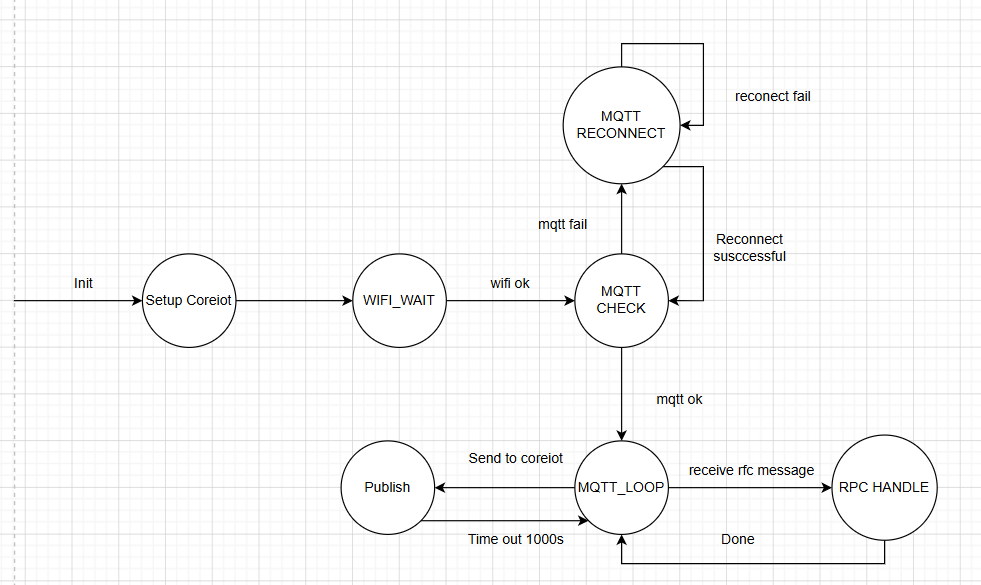
\includegraphics[width=1\linewidth]{picture/task_6_fsm.png}
\caption{Task 6 FSM}
\end{figure}

\subsection{Cấu hình Rule Chains}

Để tự động hóa quá trình giám sát và điều khiển hệ thống,sử dụng các Rule Chain nhằm xử lý dữ liệu telemetry được gửi lên từ ESP32. Hệ thống bao gồm hai luồng xử lý chính: điều khiển thiết bị thông qua RPC dựa trên nhiệt độ môi trường và gửi email cảnh báo khi nhiệt độ vượt ngưỡng cho phép.

\subsubsection{Rule Chain 1: Điều khiển cảnh báo chéo theo nhiệt độ}

Rule Chain này có nhiệm vụ phân tích dữ liệu nhiệt độ gửi từ ESP32 thứ nhất và tự động gửi lệnh RPC đến ESP32 thứ hai để điều khiển trạng thái nháy LED tương ứng với từng mức nhiệt độ.

\begin{figure}[H]
\centering
    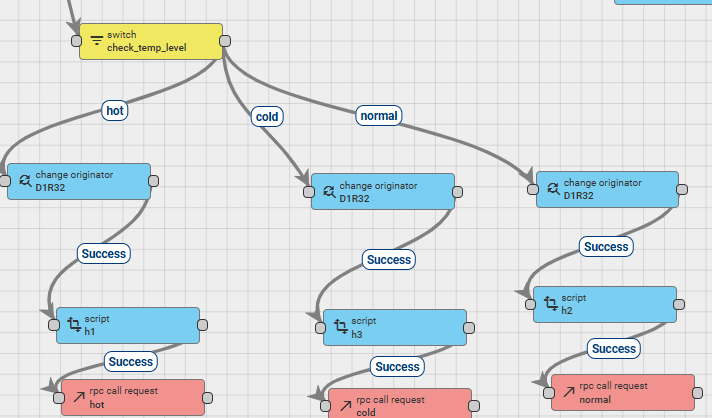
\includegraphics[width=1\linewidth]{picture/rule_tmp.png}
\caption{Sơ đồ tổng quan Rule Chain 1: Điều khiển cảnh báo qua RPC}
\end{figure}

\begin{itemize}
    \item \textbf{Phân loại nhiệt độ (Switch Node):} Hệ thống sử dụng một đoạn JavaScript trong nút Switch để kiểm tra giá trị của trường \texttt{temperature}. Dựa trên nhiệt độ đo được, dữ liệu sẽ được phân loại thành ba mức:
    \begin{itemize}
        \item \texttt{cold}: nhiệt độ dưới 20°C
        \item \texttt{normal}: nhiệt độ từ 20°C đến dưới 30°C
        \item \texttt{hot}: nhiệt độ từ 30°C trở lên
    \end{itemize}

\begin{figure}[H]
\centering
    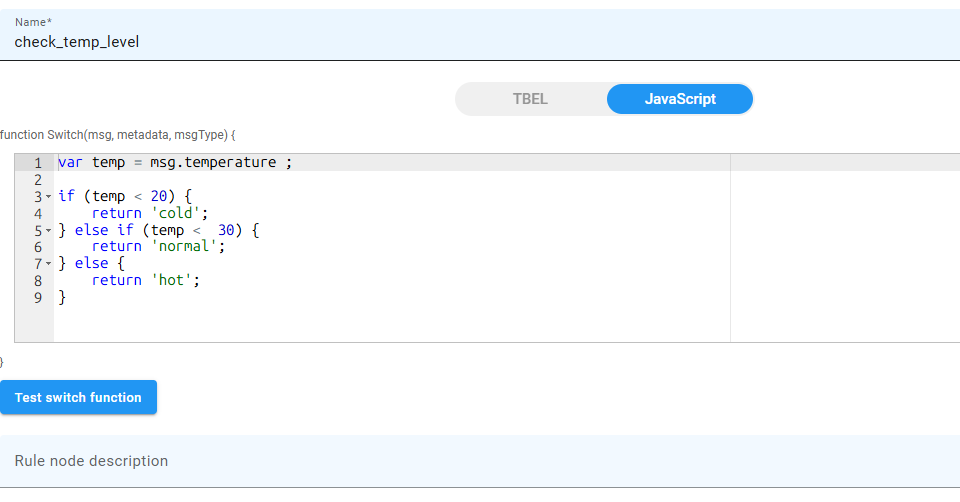
\includegraphics[width=0.8\linewidth]{picture/check_val_led.png}
\caption{Cấu hình JavaScript phân loại nhiệt độ trong nút Switch}
\end{figure}

    \item \textbf{Điều khiển thiết bị đích qua RPC:} Sau khi được phân loại, dữ liệu sẽ đi qua nhánh xử lý tương ứng để thực hiện điều khiển thiết bị theo ba bước:
    
    \begin{enumerate}
        \item \textbf{Change Originator:} Nút này thay đổi nguồn gốc của thông điệp từ ESP32 gửi dữ liệu sang ESP32 đích chứa LED cảnh báo. Điều này giúp lệnh RPC được gửi đúng đến thiết bị cần điều khiển.
        
        \item \textbf{Script:} Payload tiếp tục được xử lý tại nút Script để tạo dữ liệu điều khiển phù hợp, ví dụ như chế độ hoặc kiểu nháy LED.
        
        \item \textbf{RPC Call Request:} Cuối cùng, ThingsBoard gửi yêu cầu RPC đến ESP32 thứ hai. Thiết bị này sẽ nhận lệnh và thực hiện hiệu ứng nháy LED nhằm biểu thị trạng thái nhiệt độ hiện tại của môi trường.
    \end{enumerate}
\end{itemize}

\subsubsection{Rule Chain 2: Gửi Email cảnh báo}

Song song với cơ chế điều khiển LED, hệ thống còn triển khai một Rule Chain riêng để phát hiện các trường hợp nhiệt độ vượt ngưỡng và gửi email cảnh báo đến người dùng.

\begin{figure}[H]
\centering
    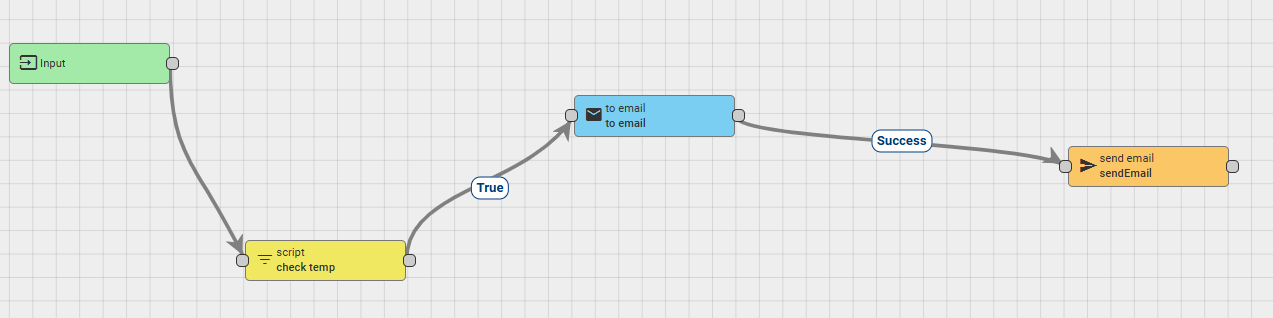
\includegraphics[width=1\linewidth]{picture/rule_mail.png}
\caption{Sơ đồ tổng quan Rule Chain 2: Gửi Email cảnh báo}
\end{figure}

\begin{itemize}
    \item \textbf{Kiểm tra điều kiện cảnh báo (Filter Node):} Dữ liệu telemetry trước tiên đi qua một nút Filter sử dụng JavaScript để so sánh nhiệt độ hiện tại (\texttt{msg.temperature}) với ngưỡng giới hạn (\texttt{msg.tempThreshold}). Nếu nhiệt độ vượt quá ngưỡng cho phép, kết quả trả về sẽ là \texttt{true} và luồng cảnh báo tiếp tục được thực hiện.

\begin{figure}[H]
\centering
    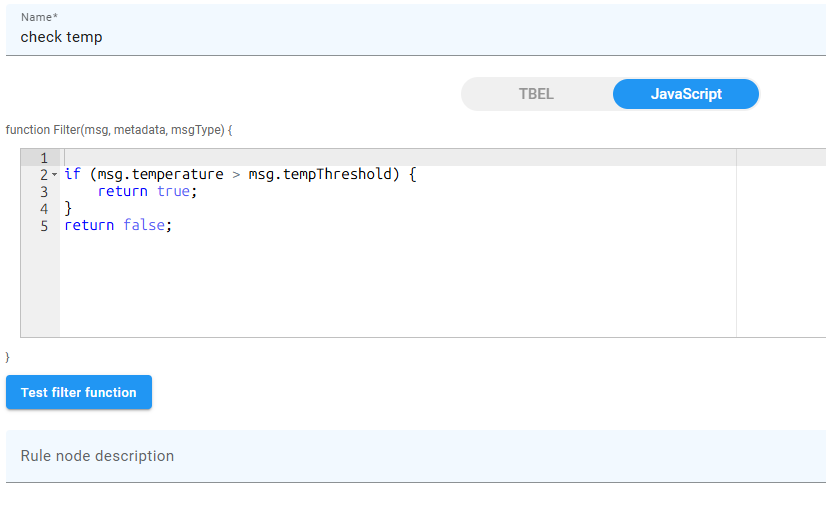
\includegraphics[width=0.9\linewidth]{picture/check_tmp_mail.png}
\caption{Bộ lọc kiểm tra điều kiện nhiệt độ vượt ngưỡng}
\end{figure}

    \item \textbf{Tạo nội dung Email (Transform Node - to email):} Khi điều kiện cảnh báo được thỏa mãn, dữ liệu sẽ được chuyển đến nút Transform để tạo nội dung email. Tại đây, hệ thống tự động sinh tiêu đề và nội dung thư bằng cách trích xuất các thông tin như tên thiết bị và giá trị nhiệt độ hiện tại. Địa chỉ email người nhận cũng được cấu hình sẵn trong node này.

\begin{figure}[H]
\centering
    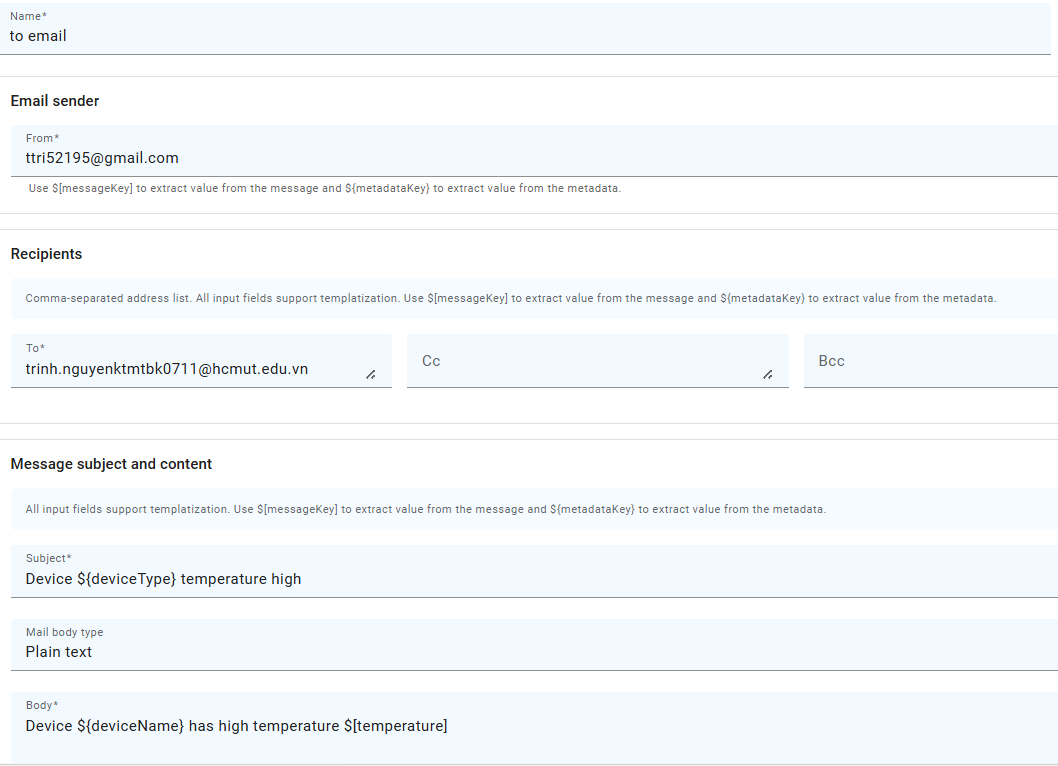
\includegraphics[width=0.9\linewidth]{picture/node_to_mail.png}
\caption{Cấu hình nội dung và người nhận Email cảnh báo}
\end{figure}

    \item \textbf{Gửi Email thông qua SMTP:} Sau khi hoàn tất định dạng nội dung, email sẽ được gửi thông qua máy chủ SMTP của Google sử dụng cổng 587 với cơ chế mã hóa TLSv1.2 nhằm đảm bảo an toàn trong quá trình truyền tải dữ liệu.

\begin{figure}[H]
\centering
    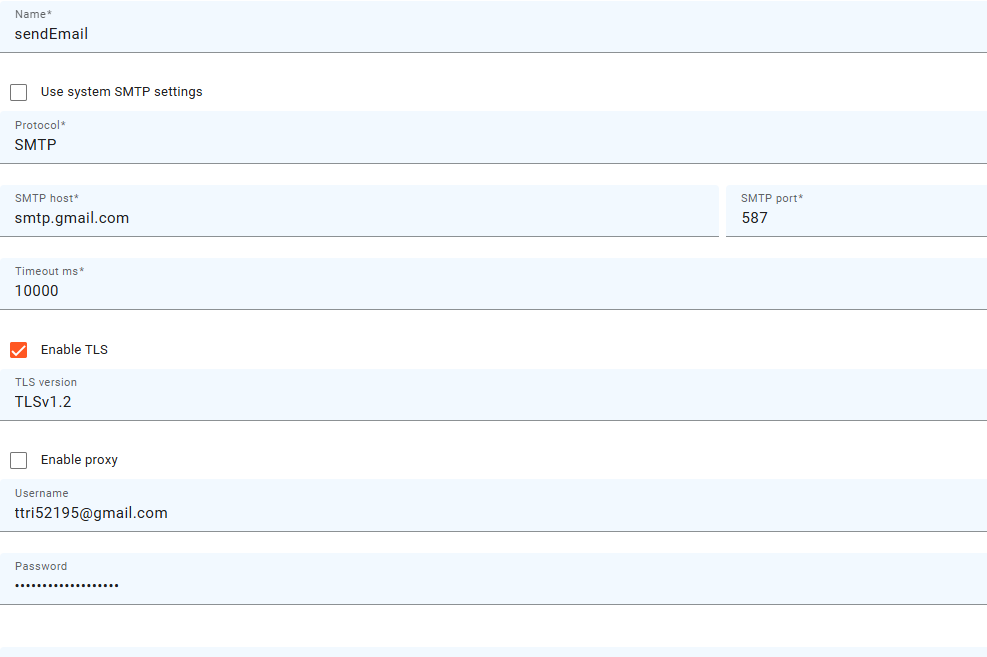
\includegraphics[width=0.8\linewidth]{picture/snd_mail.png}
\caption{Cấu hình máy chủ SMTP để gửi Email}
\end{figure}

\end{itemize}